\documentclass[a4paper,10pt]{article}

\usepackage{graphicx}
\usepackage[utf8]{inputenc}
\usepackage[spanish]{babel}
\usepackage{hyperref}
\usepackage{listings}
\usepackage{verbatim}
\usepackage[top=2cm, bottom=1.5cm, left=2.5cm, right=1cm]{geometry}
\usepackage{pdfpages}
\usepackage{enumitem}

\begin{document}
\begin{center}

{\bf{\Huge Universidad de Buenos Aires}}\\[0.5cm]
{\bf{\Huge Facultad de ingenieria}}\\[0.3cm]

{\LARGE 66.17 - Sistemas digitales}\\[1.25cm]
{\Large }Trabajo práctico Nro. 1\\[2.3cm]
{\LARGE {\bf Contador BCD de 4 dígitos con salida a display 7 segmentos}}\\[3.5cm]
{\large Lucas Simonelli}\\[2cm]
Buenos Aires - \today
\\[5.2cm]

\end{center}

% Contacto %
{Contacto: lucasp.simonelli@gmail.com}\\[2cm]
\thispagestyle{empty}   % quita el nómero en la primer pógina



\begin{comment}
\begin{abstract}
Acá va un resumen del trabajo práctico
\end{abstract}
\end{comment}

\newpage
\tableofcontents
\newpage
\section{Objetivo}
En el presente trabajo práctico se detallará el diseño, desarrollo e implementación en FPGA de un sistema digital para un voltímetro digital con salida VGA.
\section{Diagramas en bloques}
	\subsection{Diagrama general}
	\begin{figure}[h]
		\centering
		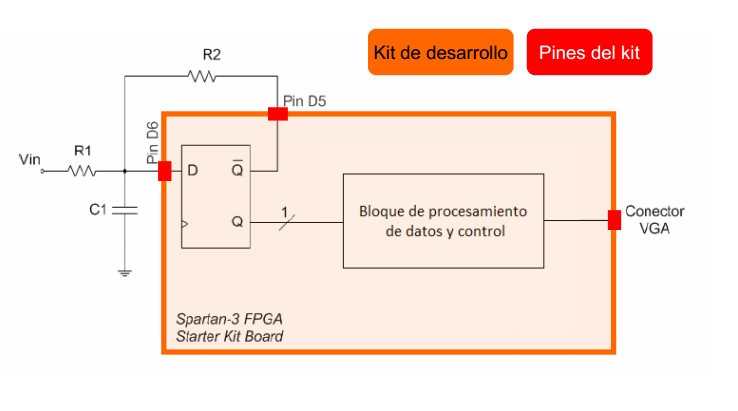
\includegraphics{img/general.png}
		\caption{Diagrama en bloques de la arquitectura propuesta por el enunciado.}
		 \label{glob}
	\end{figure}
	\subsection{Diagrama bloque procesamiento de datos y control}
		\begin{figure}[h]
		\centering
		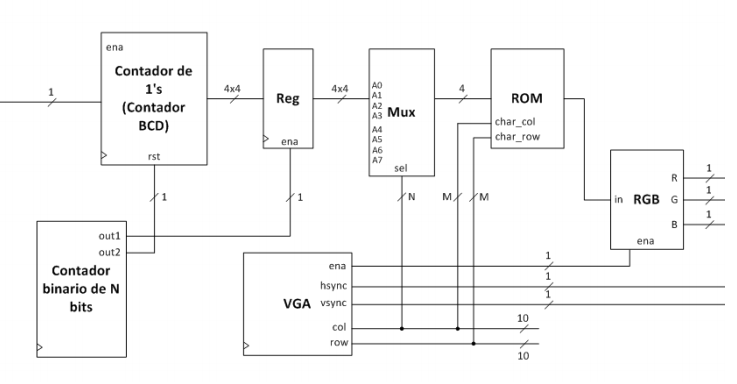
\includegraphics[width=13cm]{img/fpga.png}
		\caption{Diagrama del bloque de procesamiento.}
	\end{figure}
	
\section{Conversión A/D}

Se utilizó un conversor A/D mediante modulación Sigma/Delta, basado en el siguiente esquema:
	\begin{figure}[h]
		\centering
		\includegraphics[width=13cm]{img/sd.png}
		\caption{Conversor sigma/delta}
	\end{figure}

El circuito se implementó con dos resistencias y un capacitor, como puede verse en la figura \ref{glob}.

\section{Descripción de los componentes}
\subsection{Contador BCD}
El contador BCD de 0000 a 9999 se tomó del trabajo práctico anterior. Está implementado con 4 contadores binarios de 4 bits.

\subsection{Contador binario de N bits}\label{gen}
Este contador se implementó mediante el generador de enable utilizado en el trábajo práctico 1. Luego de N ciclos activa el registro, y en
el ciclo N+1 resetea el contador BCD y desactiva el enable del registro.

\subsection{Multiplexor}
El multiplexor se implementó mediante un process en el controlador VGA; en base a la posición actual en pantalla y el valor de la cuenta BCD almacenada en el registro, se elige el índice que corresponde al dígito almacenado en la memoria ROM.

\subsection{Controlador VGA - ROM}
Estos controladores se tomaron de la página de la materia; se agregaron los caracteres necesarios en la memoria y se modificó la integración VGA-ROM para poder mostrar varios dígitos en posiciones distintas.

\section{Tests realizadas}
Los componentes tomados del trabajo N 1 ya habían sido probados en éste. Respecto de los componentes de este trabajo, sólo se tuvo que agregar un registro, que se probó fácilmente:
	\begin{figure}[h]
		\centering
		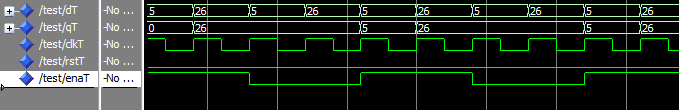
\includegraphics[width=17cm]{img/testReg.png}
		\caption{Captura de pantalla del test del registro.}
	\end{figure}
	
La integración de los bloques con el controlador VGA y la memoria ROM se testeó directamente por la pantalla.

\section{Conclusiones}
En el presente trabajó se consolidaron los conocimientos aprendidos en el  TP anterior. Se aprendió a manejar la salida VGA del FPGA y a interactuar con la memoria ROM.
\section{Resumen del output de la sintetización}
\includepdf[scale=0.8,pages={1,2}]{AplicVGA_summary.pdf}



\begin{comment}
\begin{thebibliography}{99}

\bibitem{INT06} Intel Technology \& Research, ``Hyper-Threading Technology,'' 2006, http://www.intel.com/technology/hyperthread/.

\bibitem{HEN00} J. L. Hennessy and D. A. Patterson, ``Computer Architecture. A Quantitative
Approach,'' 3ra Edición, Morgan Kaufmann Publishers, 2000.

\bibitem{LAR92} J. Larus and T. Ball, ``Rewriting Executable Files to Mesure Program Behavior,'' Tech. Report 1083, Univ. of Wisconsin, 1992.

\end{thebibliography}
\end{comment}
\end{document}
